% PROSZĘ KOMPILOWAĆ TEN DOKUMENT ZA POMOCĄ SILNIKA XELATEX
% W PRZECIWNYM RAZIE NALEŻY USUNĄĆ PAKIET fontspec ORAZ USTAWIENIA FONTU
% Z PLIKU styles/prez_wmini_pl.sty (PIERWSZE TRZY LINIJKI)
% W PRZYPADKU BRAKU FONTU Adagio Slab NALEŻY ZGŁOSIĆ SIĘ DO BIP PW O JEGO UDOSTĘPNIENIE,
% ZAŁADOWAĆ INNY KRÓJ CZCIONKI LUB ZAKOMENTOWAĆ/USUNĄĆ USTAWIENIA FONTU

\documentclass[aspectratio=169]{beamer}

\usepackage{styles/prez_wmini_pl}
\usepackage{booktabs}
\setbeamertemplate{section in toc}[sections numbered]
\setbeamertemplate{subsection in toc}[subsections numbered]
\usepackage{times}

\definecolor{quotationcolour}{HTML}{F0F0F0}
\definecolor{quotationmarkcolour}{HTML}{1F3F81}

% Double-line for start and end of epigraph.
\newcommand{\epiline}{\hrule \vskip -.2em \hrule}
% Massively humongous opening quotation mark.
\newcommand{\hugequote}{%
  \fontsize{42}{48}\selectfont \color{quotationmarkcolour} \textbf{``}
  \vskip -.5em
}

% Beautify quotations.
\newcommand{\epigraph}[2]{%
  \bigskip
  \begin{center}
  \colorbox{quotationcolour}{%
    \parbox{.80\textwidth}{%
    \epiline \vskip 1em {\hugequote} \vskip -.5em
    \parindent 2.2em
    #1\begin{flushright}\textsc{#2}\end{flushright}
    \epiline
    }
  }
  \end{center}
  \bigskip
}

\newcommand{\boldm}[1] {\mathversion{bold}#1\mathversion{normal}}

\graphicspath{ {./images/} }



% ------------------ Ustawienia użytkownika ------------------
% kolor tytułu prezentacji; zalecany white lub grafitowy.
% Poza tym można użyć zdefiniowanych w pakiecie kolorów:
% sloneczny, morelowy, mietowy, mokka, grafitowy, sliwkowy, szafirowy, wrzosowy
% lub wybrać sobie kolor z pakietu xcolor
\colorlet{title_color}{grafitowy}

\title{Opracowanie wirtualnego środowiska\\do symulacji dynamiki lotu\\ bezzałogowych statków powietrznych}
%\subtitle{Podtytuł consectetur adispiscing elit}
\author{Wojciech Gajda \and  Igor Faliszewski}
\date{28 listopada 2023} % można tam wpisać datę jaką się chce lub zakomentować dla daty dzisiejszej



% ------------------ Początek prezentacji ------------------

\begin{document}
\sloppy

% Slajd tytułowy
{
\maketitleframe 
}

\begin{frame}
\frametitle{Agenda}
  \tableofcontents[  
    sectionstyle=show, 
    %hideallsubsections
    ]
\end{frame}

\section{Wprowadzenie}
\subsection{Motywacje}
\begin{frame}%[allowframebreaks]
	\frametitle{Motywacja}
	\begin{columns}
		\begin{column}{0.33\textwidth}
	   	 	\begin{figure}
	   		 \centering
	      		 \uncover<2->{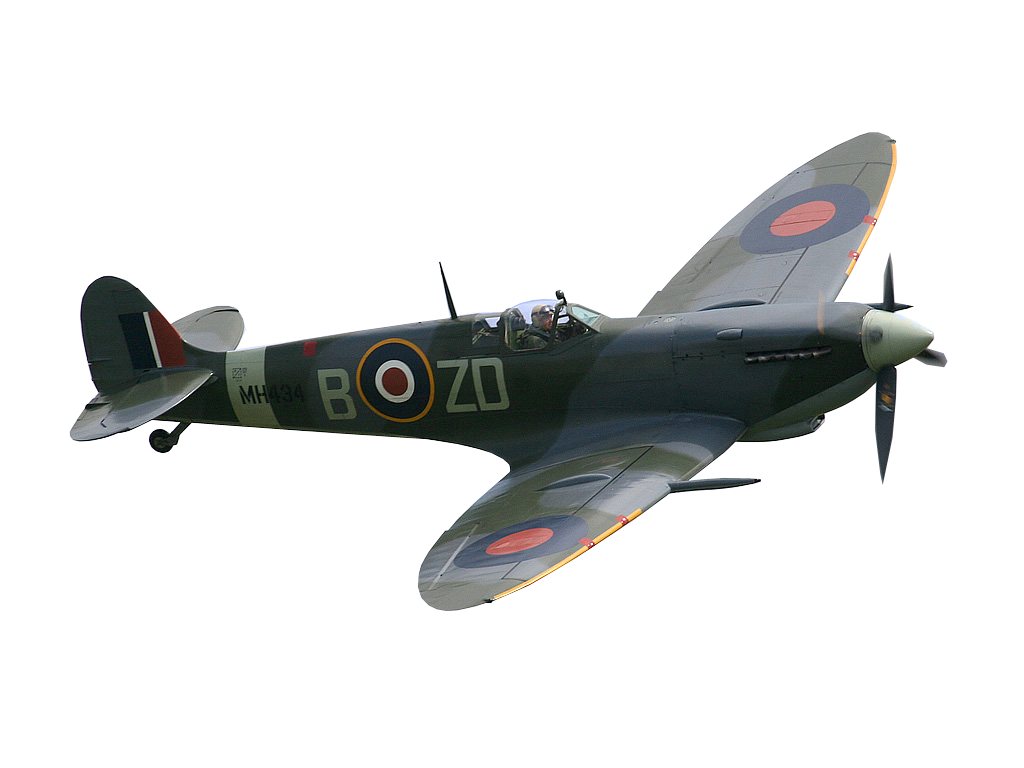
\includegraphics[width=0.9\textwidth]{spitfire.png}}
	    		\end{figure}
		\end{column}
		\begin{column}{0.33\textwidth}
	   	 	\begin{figure}
	   		 \centering
	      		 \uncover<3->{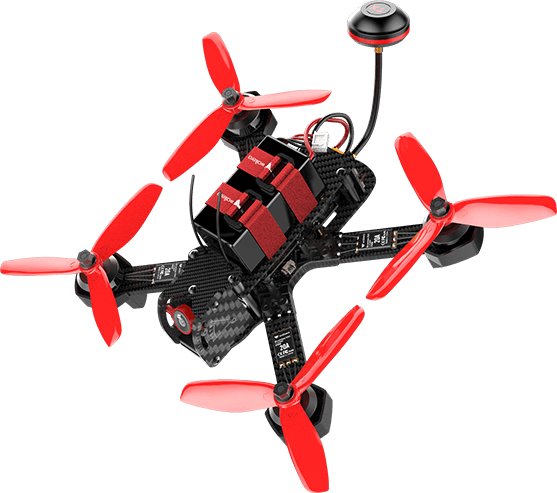
\includegraphics[width=0.9\textwidth]{quadcopter_fpv.png}}
	    		\end{figure}
		\end{column}
		\begin{column}{0.33\textwidth}
	    		\begin{figure}
	   		 \centering
	      		 \uncover<4->{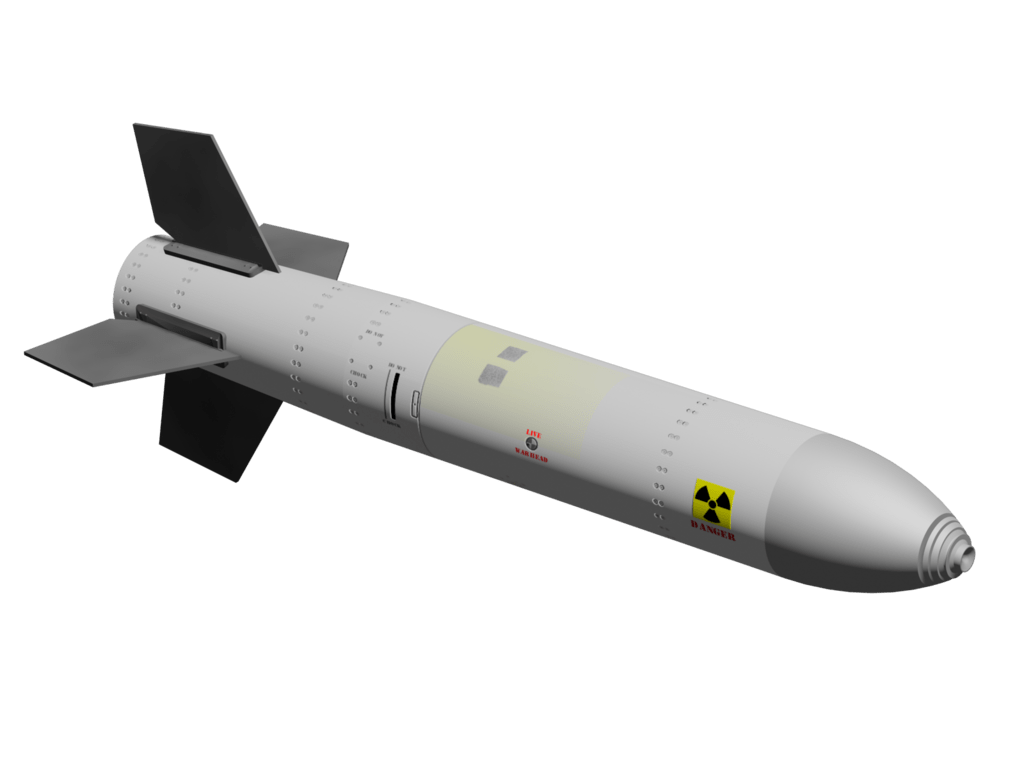
\includegraphics[width=0.9\textwidth]{missile.png}}
	    		\end{figure}
		\end{column}
	\end{columns}
	\begin{figure}
		\hfill
		\uncover<5->{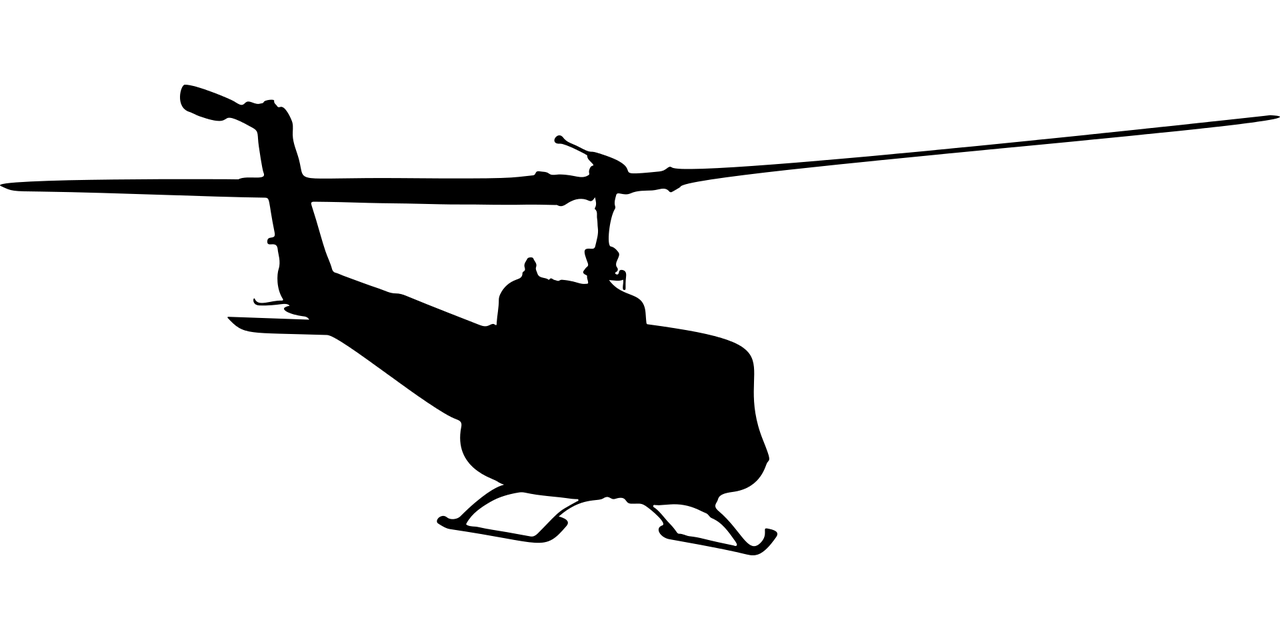
\includegraphics[width=0.2\textwidth]{helicopter.png}}
	\end{figure}
\end{frame}

\subsection{Cel projektu}
\begin{frame}%[allowframebreaks]
	\frametitle{Cel projektu}
	  \begin{itemize}
	  \item {
	    Kompleksowa symulacja fizyki.
	    \pause % Tu nastąpi pauza
	  }
	  \item {   
	    Wysoka konfigurowalność BSP, środowiska i symulacji.
	  }
	  % Można ustalić kiedy dany element ma się pojawić, używając <n->:
	  \item<3-> {
	    Bogate narzędzia dla analityków.
	  }
	  \item<4-> {
	    Licencja open-source.
	  }
 	 \end{itemize}
\end{frame}

\section{Wstep teoretyczny}
\begin{frame}%[allowframebreaks]
	\frametitle{Wstep teoretyczny}
	\epigraph{Nie ma osobnej ani teorii, ani praktyki inżynierskiej, jest tylko wspólna sztuka inżynierska}{prof. Jan Oderfeld}
\end{frame}


\subsection{Dynamika statku powietrznego}
\begin{frame}[allowframebreaks]
	\frametitle{Dynamika lotu}
	
\end{frame}

\begin{frame}[allowframebreaks]
	\frametitle{Równania stanu}
	
\end{frame}

\begin{frame}[allowframebreaks]
	\frametitle{Równania różniczkowe}
	
\end{frame}

\begin{frame}[allowframebreaks]
	\frametitle{Model matematyczny statku powietrznego}
	
\end{frame}

\begin{frame}[allowframebreaks]
	\frametitle{Kolizje}
	
\end{frame}

\begin{frame}[allowframebreaks]
	\frametitle{Odrzut}
	
\end{frame}

\subsection{Sterowanie statkiem powietrznym}
\begin{frame}[allowframebreaks]
	\frametitle{Sterowanie statkiem powietrznym}
\end{frame}

\begin{frame}[allowframebreaks]
	\frametitle{Nawigacja}
	
\end{frame}

\begin{frame}[allowframebreaks]
	\frametitle{Regulatory PID}
	
\end{frame}

\subsection{Grafika komputerowa}

% Wprowadzając grafikę komputerową, nie można nie wpsomnieć o GPU, a więc procesorach graficznych. Jak nazwa wskazuje zostały one początkowo wprowadzone na rynek by programy były sobie w stanie radzić z wykonywaniem rzędy wielkości operacji więcej niż to co jest możliwe na zwykłym procesorze. 
\begin{frame}
\frametitle{GPU}
	\begin{figure}
		\centering
		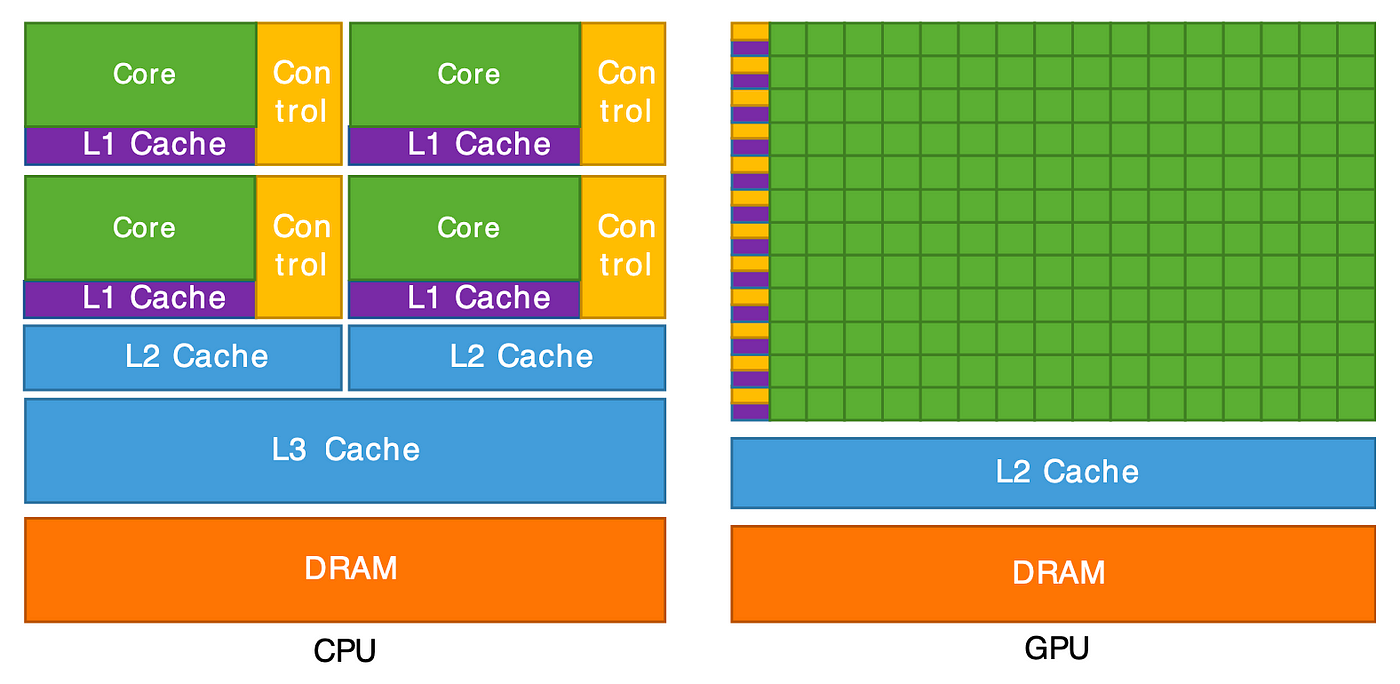
\includegraphics[width=0.8\textwidth]{gpu.png}
	\end{figure}
\end{frame}

% OpenGL czyli Open Graphics Libraru, jest uniwersalnym interfejsem do renderowania grafiki werktorowej 2D i 3D wykorzystującym GPU. Za specyfikację OpenGL odpowiada Khronos Group, a za implementację funkcji najczęściej producenci kart graficznych. W praktyce jest to olbrzymia maszyna stanu, która definiuje sposób działania OpenGL. Aby stan zmieniać operujemy na obiektach, które przypisujemy do kontekstu. [Opisać obrazek]
\begin{frame}
\frametitle{OpenGL}
	\begin{figure}
		\centering
		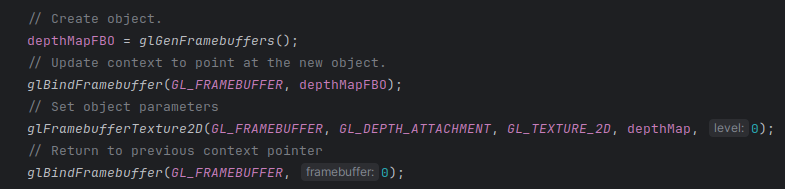
\includegraphics[width=0.9\textwidth]{OpenGL_example.png}
	\end{figure}
\end{frame}

% Przetwarzanie wierzchołków
% Każdy obiekt w scenie składa się z wierzchołków. Atrybuty tych wierzchołków (np. położenie) poddawane są przekształceniom. []Narysować dwa obiekty takie same jak przechodzą na płaszczyznę ekran]. (Mamy na to wpływ w Vertex Shader)
% Łączenie w prymitywy
% [Pokazać trójkąty]
% Przycinanie
% Rasteryzacja
% Tworzone są fragmenty, czyli próbki powierzchni prytmitywu, któremu odpowiada piksel bufora klatki. Może być wiele fragmentów na jeden piksel. W tym momencie dane wierzchołka są interpolowane, w przypadku trójkąta, z trzech wierzchołków. 
% Przetwarzanie fragmentów.
% Dodawanie tekstury, oświetlenie. (Mamy na to wpływ w Fragment Shader)
% Przetwarzanie piksli
% Tutaj zachodzi test głębokości, alpha blending czyli przezroczystość i antialiasing.

% Teraz opiszemy to na co mamy wpływ, a więc dane, przetwarzanie wierzchołków i fragmentów.
\begin{frame}
\frametitle{Potok renderowania}
		\begin{figure}
			\centering
			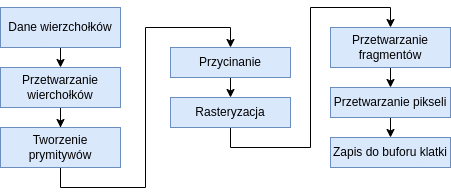
\includegraphics[width=0.7\textwidth]{graphics_pipeline.png}
		\end{figure}
\end{frame}

% Porozumiewanie się z procesrowem graficznym wymaga jednak własnego języka. W przypadku OpenGLa, jest nim GLSL ,,OpenGl Shading Language''. Został on zaprojektowany na bazie C, nakładając duży poziom abstrakcji na operacje wykonywane na GPU. Pisząc shadery właściwie się nie myśli o równoległości. [Opis języka]
\begin{frame}[allowframebreaks]
	\frametitle{Shadery}
	\begin{figure}
		\centering
		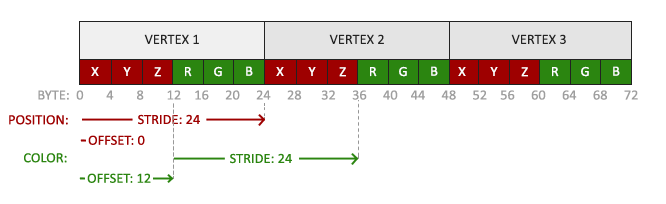
\includegraphics[width=0.8\textwidth]{vertex_attributes.png}
	\end{figure}
	\framebreak
	
	\begin{figure}
		\centering
		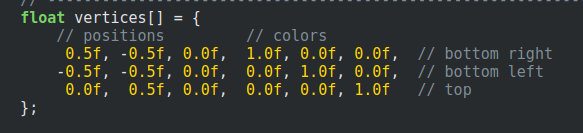
\includegraphics[width=0.8\textwidth]{vertex.png}
	\end{figure}
	\framebreak
	
	\begin{columns}
		\begin{column}{0.5\textwidth}
			\begin{figure}
				\centering
				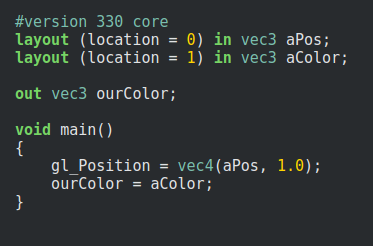
\includegraphics[width=0.9\textwidth]{vertex_shader.png}
			\end{figure}
		\end{column}	
		
		\begin{column}{0.5\textwidth}
			\begin{figure}
				\centering
				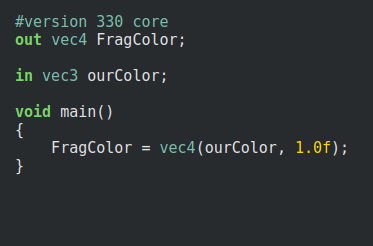
\includegraphics[width=0.9\textwidth]{fragment_shader.png}
			\end{figure}
		\end{column}
	\end{columns}
	\framebreak
	
	\begin{figure}
	\centering
	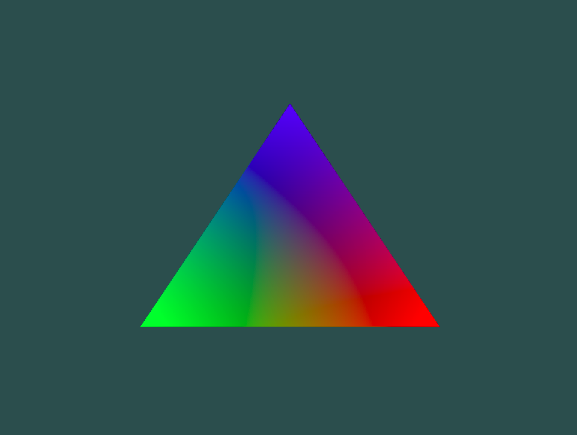
\includegraphics[width=0.6\textwidth]{shader_result.png}
	\end{figure}
\end{frame}

% Cieniowanie w grafice komputerowej możemy wykonywać na różne sposoby. 
% Od lewej mamy:
% Kolorowanie płaskie - tutaj oświetlenie ustalamy na poziomie prymitywu.
% KOlorwanie Gourauda - Tutaj ustalamy oświetlenie na poziomie wierzchołków i je interpolujemy.
% Kolorowanie Phonga - Tutaj interpolujemy wektory normalne. Obliczenie koloru następuje dla każdego fragmentu.
\begin{frame}[allowframebreaks]
	\frametitle{Cieniowanie i model oświetlenia}	
	\begin{figure}
		\centering
		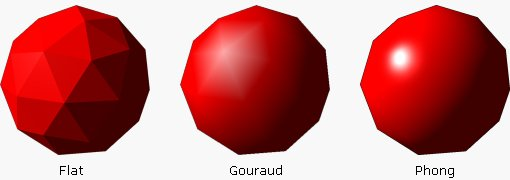
\includegraphics[width=0.7\textwidth]{shading.jpg}
	\end{figure}
	\framebreak
	\begin{figure}
		\centering
		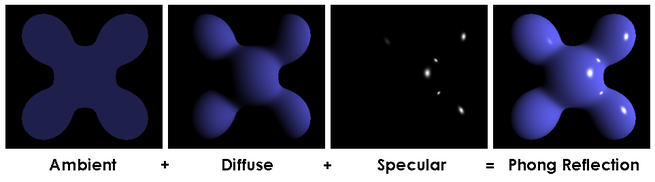
\includegraphics[width=0.9\textwidth]{phong.png}
	\end{figure}
\end{frame}

% \begin{frame}[allowframebreaks]
% 	\frametitle{Renderowanie interfejsu}
%	
% \end{frame}

% Istotnym elementem symulacji jest również interakcja z użytkownikiem.
% W naszym przypadku większość komunikacji odbywa się za pomocą kontrolera.
% System interpretuje każdy kontroler jako tablicę stanów przycisków, osi oraz hatów (d-padów).
% Niestety za jakie przyciski odpowiadają jakie indeksy, nie wiadomo. Zależy to od producenta kontrolera i trudno jest o jakiś standard w przypadku tylu różnych możliwości układu przycisków. 
% Są bazy danych, które pozwalają na mapowanie znanych modeli kontrolerów do konkretnych akcji, ale my chcemy umożliwić wykrozystanie najróżniejszych sprzętów. Od zwykłego pada do xboxa, po dedykowany kontroler do BSP.
% Rozwiązanie tego problemu nie jest takie trudne, chociaż pracochłonne. Wystarczy stworzyć interaktywną konfigurację, z której pomocą użytkownik sam będzie w stanie ustawić dedykowane bindingi.
\begin{frame}[allowframebreaks]
	\frametitle{Obsługa kontrolera}
	
	\begin{columns}
		\begin{column}{0.33\textwidth}
			\begin{figure}
				\centering
				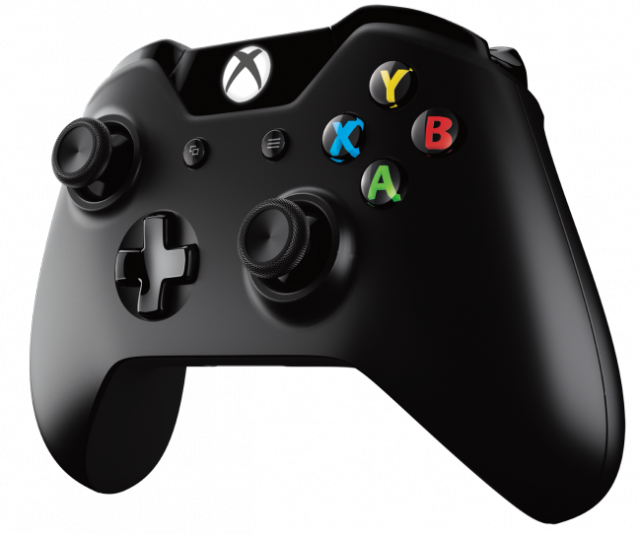
\includegraphics[width=0.7\textwidth]{xobx.png}
			\end{figure}
		\end{column}
		\begin{column}{0.33\textwidth}
			\begin{figure}
				\centering
				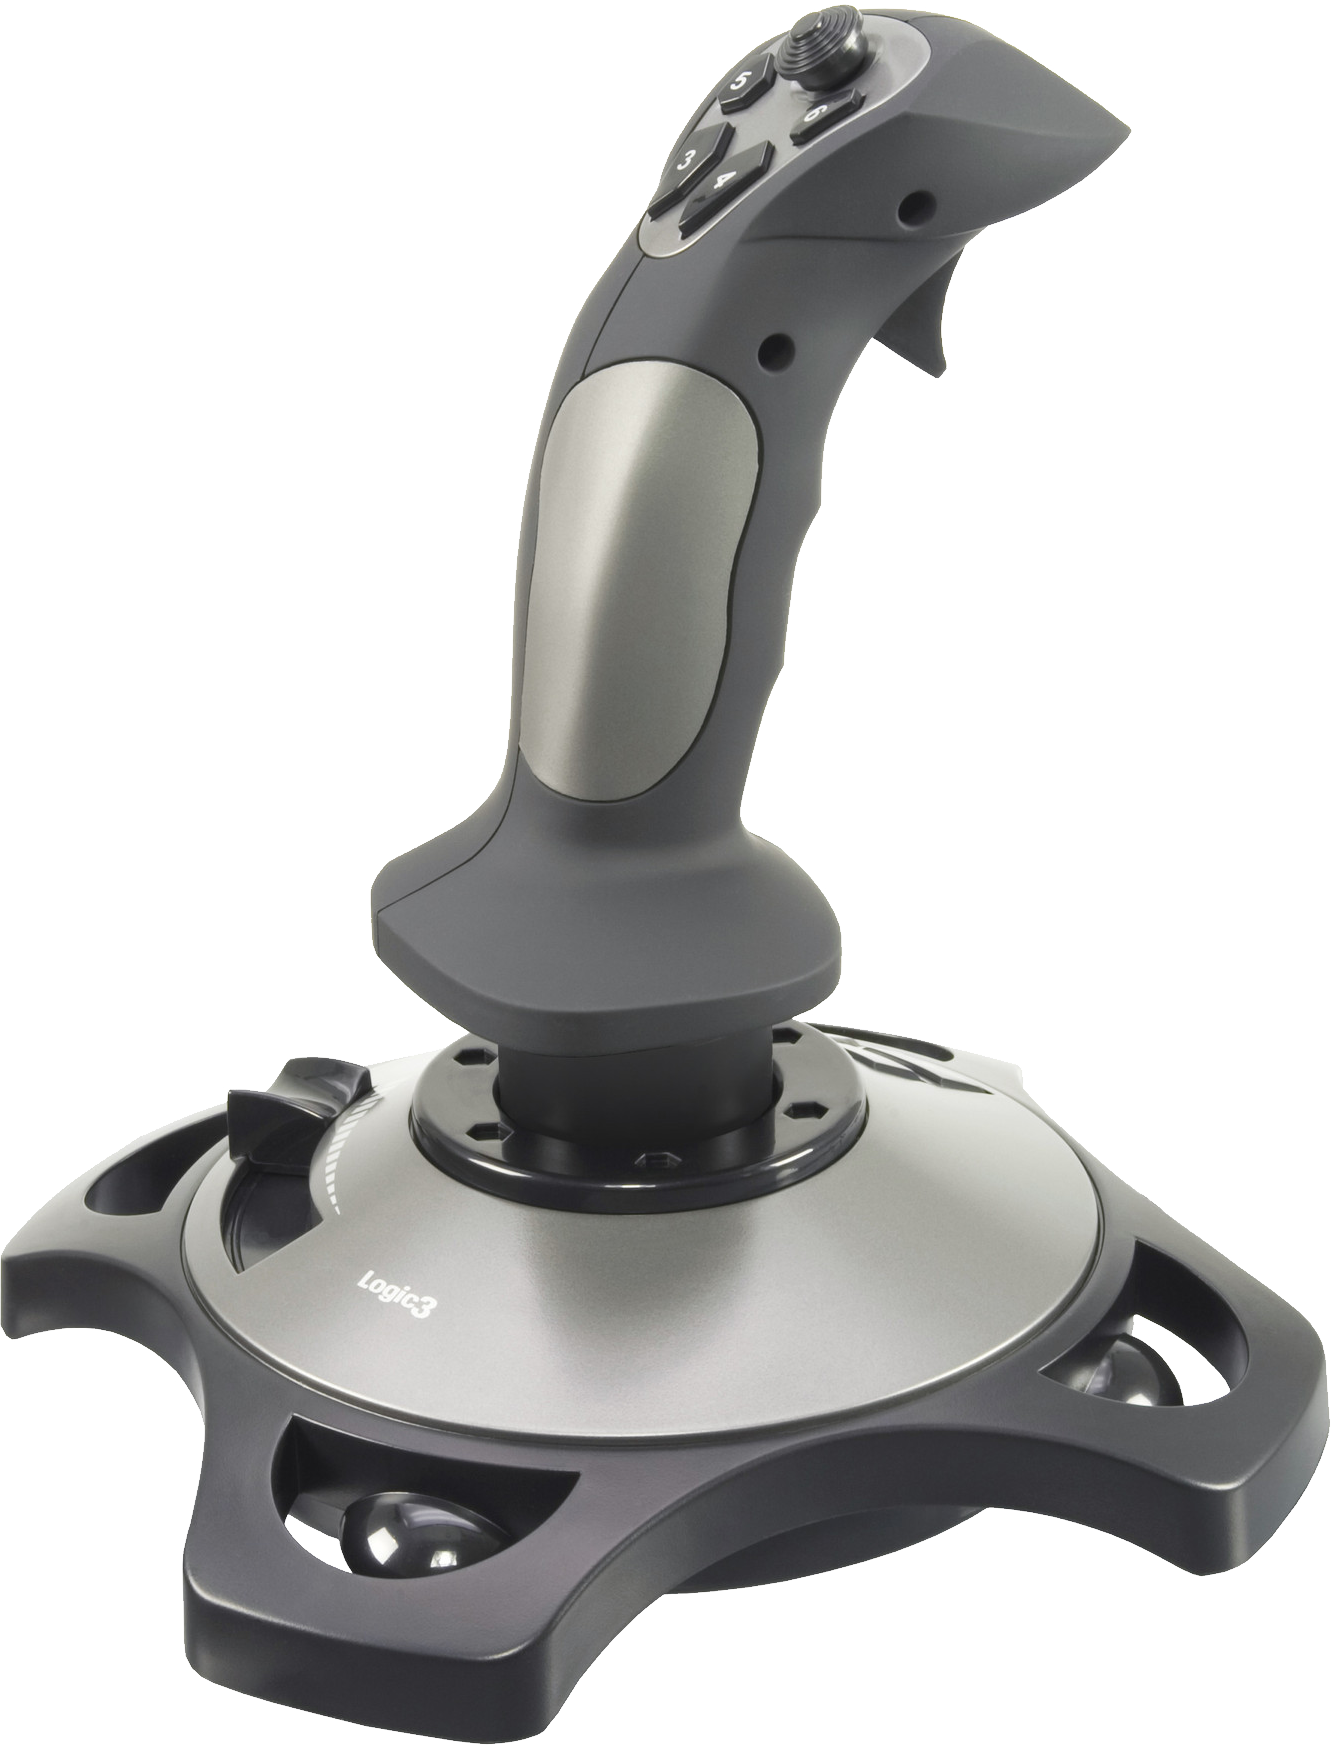
\includegraphics[width=0.7\textwidth]{joysticke.png}
			\end{figure}
		\end{column}
		\begin{column}{0.33\textwidth}
			\begin{figure}
				\centering
				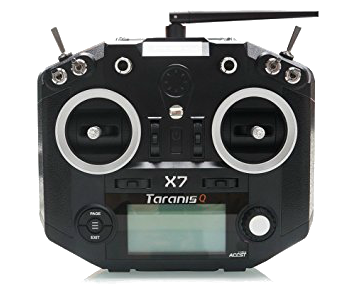
\includegraphics[width=0.7\textwidth]{taranis.png}
			\end{figure}
		\end{column}
	\end{columns}
	
	\begin{figure}
		\centering
		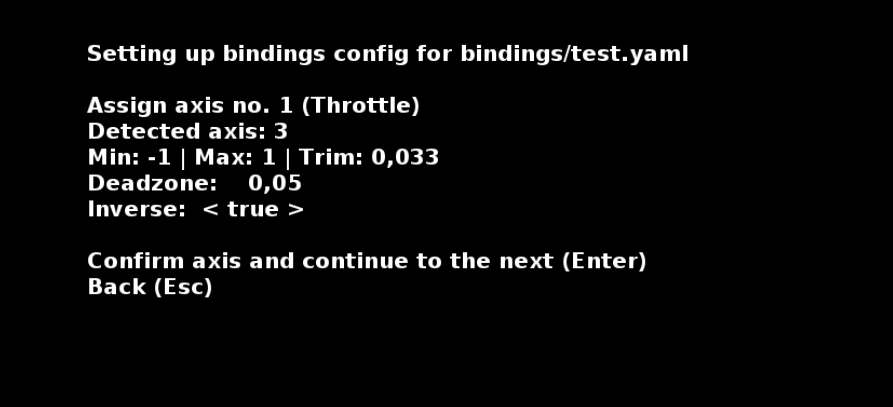
\includegraphics[width=0.8\textwidth]{bindings.png}
	\end{figure}
\end{frame}

\begin{frame}[allowframebreaks]
	\frametitle{Krzywa łańcuchowa}
	\begin{figure}
		\centering
		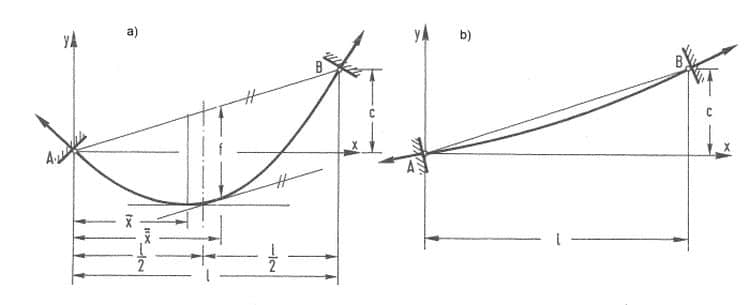
\includegraphics[width=0.7\textwidth]{catenary.jpg}
	\end{figure}
	$$\text{cat}(x) = a\cdot \cosh \left(\frac{x}{a}\right).$$
	
	\framebreak
	
	Wyznaczenie współczynnika krzywej łańcuchowej $a_c$ między punktami $A = (x_1,y_1)$, $B = (x_2,y_2)$ i danego $l < \lVert B - A \rVert$, to rozwiązanie równania:
	\begin{equation}
		\label{cat}
		\frac{1}{h} \sqrt{l^2-v^2} = \frac{2a_c}{h} \sinh\left( \frac{h}{2a_c} \right),
	\end{equation}
	gdzie:
	$$
	v = x_2 - x_1,
	$$
	$$
	h = y_2 - y_1.
	$$
	
	\framebreak
	Dla $l \geq \lVert B - A \rVert$ stosowany jest wzór na współczynnik kierunkowy prostej
	\begin{equation}
		\label{line}
		a_l = \frac{y_2 - y_1}{x_2 - x_1}.
	\end{equation}
	
	
	\framebreak
	Ostatecznie, dla danej długości liny $l \in \mathbb{R}$ oraz punktów $A$, $B  \in \mathbb{R}^2$ funkcja liny $f_l$ ma postać:
	$$f_l(x) = 
	\begin{cases}
		a_c \cdot \cosh\left( \frac{x}{a_c} \right), & l < \lVert B - A \rVert \\
		a_l \cdot x, & l \geq \lVert B - A \rVert 
	\end{cases},$$
	gdzie $a_c$ oraz $a_l$ są wyznaczone z równań \ref{cat} oraz \ref{line} dla punktów $A$ i $B$.
	
	\framebreak
	
	\begin{figure}
		\centering
		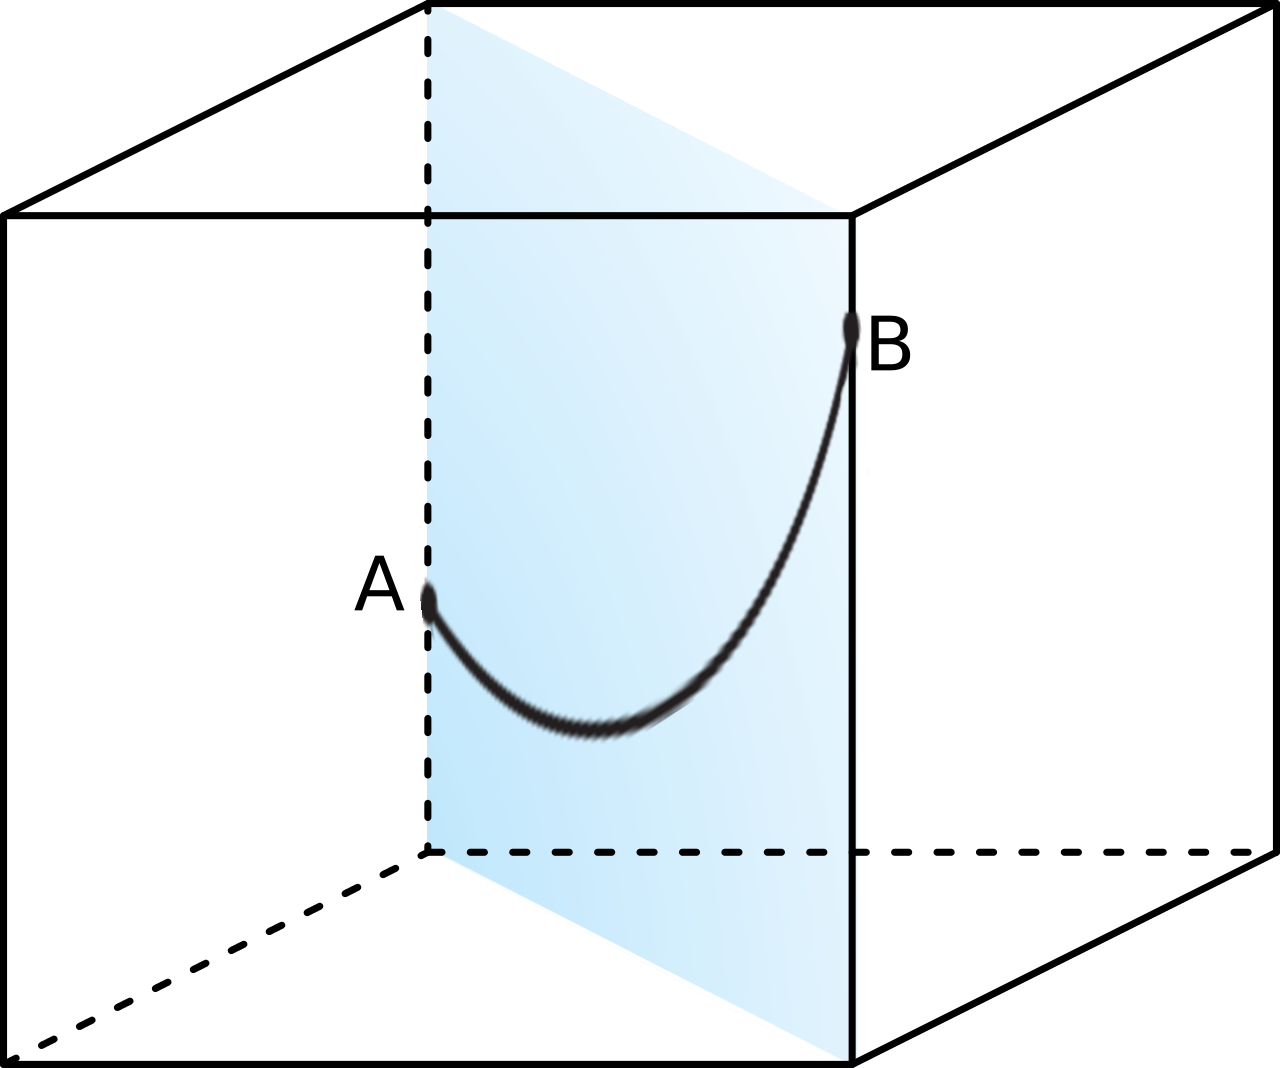
\includegraphics[width=0.4\textwidth]{cube.png}
	\end{figure}
	\framebreak
	
	
	\begin{columns}
		\begin{column}{0.5\textwidth}
			\begin{figure}
				\centering
				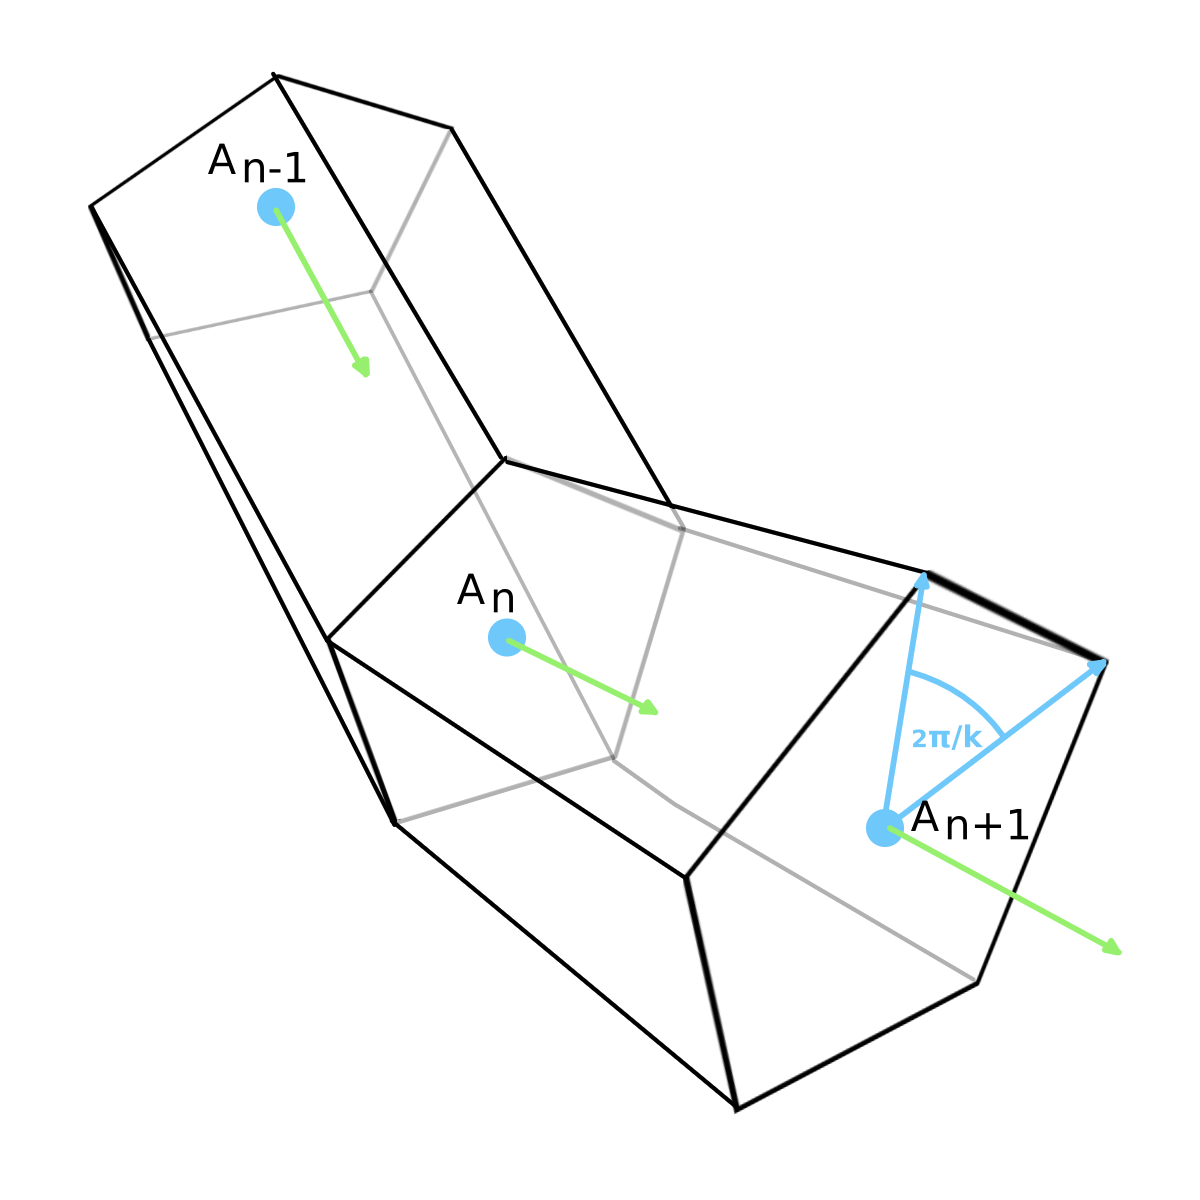
\includegraphics[width=1\textwidth]{rope_model.png}
			\end{figure}
		\end{column}	
		
		\begin{column}{0.5\textwidth}
				\begin{equation*}
				\frac{d}{dx} \text{cat}(x) = \frac{d}{dx} \left( a\cdot \cosh\left( \frac{x}{a} \right) \right) = \sinh\left( \frac{x}{a} \right)
			\end{equation*}
			\begin{equation*}
				\vec{t} =
				\begin{bmatrix}
					1 \cdot \frac{|\vec{l_x}|}{\vec{|l_{xy}}|}, &
					1 \cdot \frac{|\vec{l_y}|}{\vec{|l_{xy}}|}, &
					-\sinh(\frac{(x+x_{offset})}{a})
				\end{bmatrix}^T
			\end{equation*}
			\begin{equation*}
			\vec{n_0} =
			\begin{bmatrix}
				\sinh(\frac{(x+x_{offset})}{a}) \cdot \frac{|\vec{l_x}|}{\vec{|l_{xy}}|}, &
				\sinh(\frac{(x+x_{offset})}{a}) \cdot \frac{|\vec{l_y}|}{\vec{|l_{xy}}|}, &
				1
			\end{bmatrix}^T
			\end{equation*}
			\begin{equation*}
				M_R = 
				\begin{bmatrix}
					0 & -\vec{t_z} & \vec{t_y} \\
					\vec{t_z} & 0 & -\vec{t_x} \\
					\vec{t_y} & \vec{t_x} & 0 \\
				\end{bmatrix}
			\end{equation*}
			\begin{equation*}
				\vec{n_i} = 1 \cdot M_R^i
			\end{equation*}
		\end{column}
	\end{columns}
	\framebreak
	
\end{frame}

\section{Demo}

\begin{frame}
	  \begin{center}
	\Huge Demo
	\end{center}
\end{frame}


\begin{frame}
	\frametitle{Testy $\alpha$} %JOKE
	\begin{figure}
		\centering
		
\includegraphics[width=0.7\textwidth]{dog.jpg}
	\end{figure}
\end{frame}


\begin{frame}
	\frametitle{Dyskusja}
	\begin{figure}
		\centering
		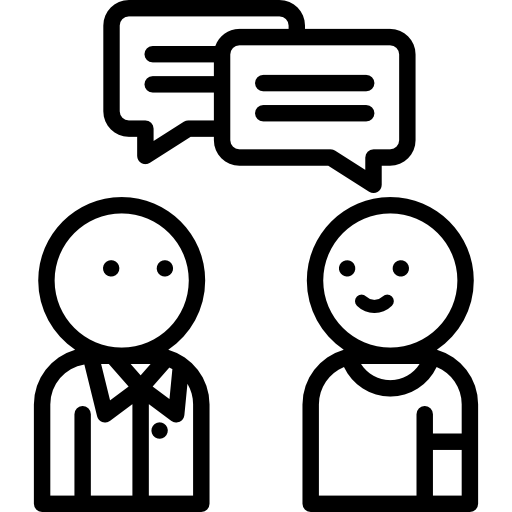
\includegraphics[width=0.7\textwidth]{questions.png}
	\end{figure}
\end{frame}

\begin{frame}
	  \begin{center}
	\Huge Dziękuje za uwagę!
	\end{center}
\end{frame}

% https://learnopengl.com/
% https://chodor-projekt.net/encyclopedia/statyka-ciegna/

\end{document}